\section{Flight cases, load cases and conventions}
\label{sec:conventions}

This section defines the cases and the signs used in the rest of the report.

\subsection{Two flight cases}

Both designs are flown with the team's Python flight model (report~2), in two cases:
\begin{itemize}
\item \textbf{Nominal day}: standard atmosphere, \SI{15}{\celsius} on the pad, propellant mass from the
total impulse.
\item \textbf{Hot day}: \SI{30}{\celsius} on the pad and the LVO masses. The rocket is lighter and
faster, so the air loads and the heating are higher. The hot day is the worst case for every value in
this report.
\end{itemize}
Speed and dynamic pressure peak at burnout, 9.1\,s after lift-off (Figure~\ref{fig:flight}).

\begin{figure}[H]
\centering
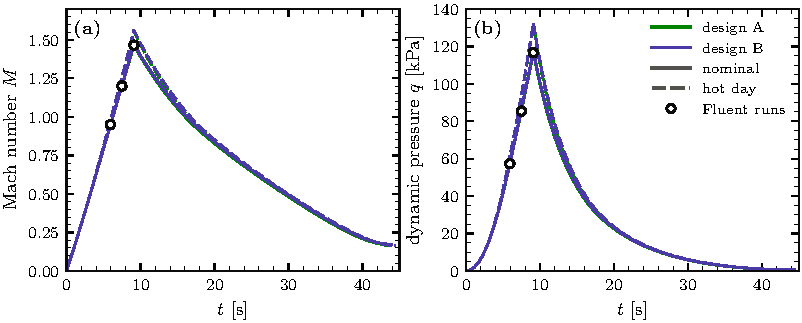
\includegraphics[width=0.9\linewidth]{fig_flight}
\caption{Mach number (a) and dynamic pressure (b) during the flight. Solid: nominal day; dashed: hot day.
The circles mark the three Fluent runs.}
\label{fig:flight}
\end{figure}

\subsection{Three load cases}

Three moments of the flight cover the largest air loads (Table~\ref{tab:lcs}).

\begin{table}[H]
\centering
\caption{The three load cases. Values for design A on a nominal day; design B differs by less than
0.5\,s. On a hot day burnout is reached at $M = \val{A-hot-LC1-M}$ and $q = \val{A-hot-LC1-q}$\,kPa.}
\label{tab:lcs}
\small
\begin{tabularx}{\linewidth}{@{}lcccc>{\raggedright\arraybackslash}X@{}}
\toprule
Load case & Time & Mach & Dynamic & Outside & Critical for\\
 & [s] & & pressure [kPa] & pressure [kPa] & \\
\midrule
\textbf{LC1, burnout} & \val{A-nominal-LC1-t} & \val{A-nominal-LC1-M} & \val{A-nominal-LC1-q} & \val{A-nominal-LC1-pinf} &
inward pressure on the tip, drag, side force and heating\\
\addlinespace
\textbf{LC2, transonic} & \val{A-nominal-LC2-t} & \val{A-nominal-LC2-M} & \val{A-nominal-LC2-q} & \val{A-nominal-LC2-pinf} &
the flow pattern changes near Mach~1; loads lower than at LC1\\
\addlinespace
\textbf{LC3, apogee} & \val{A-nominal-LC3-t} & \val{A-nominal-LC3-M} & \val{A-nominal-LC3-q} & \val{A-nominal-LC3-pinf} &
lowest outside pressure: outward pressure and pull-off force of the sealed nose\\
\bottomrule
\end{tabularx}
\end{table}

\subsection{The sealed nose}

The nose has no vent holes, so the air inside keeps the pressure it had on the pad,
$p_{pad} = \val{pad-p}$\,kPa. When the shell heats this air, its pressure rises:
\begin{equation}
p_{in} = p_{pad}\,\frac{T_{in}}{T_{pad}}.
\label{eq:dp}
\end{equation}
The temperature of the inside air $T_{in}$ is not computed. Two bounds are used instead:
\begin{itemize}
\item \textbf{cold inside air}, $T_{in} = T_{pad}$: lowest inside pressure, so the largest
\emph{inward} load;
\item \textbf{heated inside air}, $T_{in}$ = mean temperature of the inner face of the shell: highest
inside pressure, so the largest \emph{outward} load.
\end{itemize}
Each table says which bound it uses.

\subsection{Sign conventions}

Figure~\ref{fig:conventions} shows the conventions used everywhere in this report.
\begin{itemize}
\item $x$ is the distance from the tip along the axis. Four stations are followed during the flight:
the tip, 50\,mm, mid-length (half the curved part) and the shoulder (end of the curved part, where the
coupler starts).
\item The \textbf{net pressure} on the shell is $\Delta p = p_w - p_{in}$: the pressure on the outside of
the wall minus the pressure inside. $\Delta p > 0$ pushes the shell \textbf{inward}; $\Delta p < 0$ pushes
it \textbf{outward}.
\item An \textbf{axial force} $> 0$ is compression: it pushes the nose aft onto the joint. An axial
force $< 0$ is tension: it pulls the nose forward, off the joint.
\end{itemize}

\begin{figure}[H]
\centering
\begin{tikzpicture}[x=1cm, y=1cm, >={Stealth[length=2.2mm]},
  declare function={rr(\t) = 1.5*sqrt(max(0, (rad(acos(1 - 2*\t)) - 0.5*sin(2*acos(1 - 2*\t)))/pi));}]
  \def\xs{11.3}  % end of the curved part (60 mm per cm)
  \def\xj{12}    % joint plane, 720 mm
  % body tube behind the joint
  \draw[black!35] (\xj,1.5) -- (13.3,1.5) (\xj,-1.5) -- (13.3,-1.5);
  \node[black!50, font=\small] at (12.68,0) {body};
  % nose
  \filldraw[fill=black!5, draw=black, thick]
    plot[domain=0:1, samples=80, smooth] ({\xs*\x}, {rr(\x)}) -- (\xj,1.5) -- (\xj,-1.5)
    -- plot[domain=1:0, samples=80, smooth] ({\xs*\x}, {-rr(\x)}) -- cycle;
  % joint plane
  \draw[dashed, black!60] (\xj,-1.85) -- (\xj,1.9) node[above, font=\small, black!70] {joint};
  % inside air
  \node[font=\small, align=center] at (8.4,0) {air sealed at\\pad pressure, $p_{in}$};
  % flight direction
  \draw[->, black!55] (-0.2,1.0) -- (-1.2,1.0) node[midway, above, font=\small] {flight};
  % inward pressure on the front
  \foreach \px in {0.5, 1.2, 2.0}
    \draw[->, inward, thick] (\px, {rr(\px/\xs) + 0.75}) -- (\px, {rr(\px/\xs) + 0.05});
  \draw[->, inward, thick] (-0.9,0) -- (-0.07,0);
  \node[inward, font=\small, anchor=south, align=center] at (1.2,1.55) {$\Delta p > 0$\\pushes the shell in};
  % outward pressure on the rest of the shell
  \foreach \px in {5.5, 7.0, 8.5, 10.0}
    \draw[->, outward, thick] (\px, {rr(\px/\xs) + 0.05}) -- (\px, {rr(\px/\xs) + 0.75});
  \node[outward, font=\small, anchor=south, align=center] at (7.75,2.3) {$\Delta p < 0$\\pushes the shell out};
  % side force at the centre of pressure (design A)
  \draw[->, very thick] (4.92,-0.7) -- (4.92,0.7);
  \node[font=\small, anchor=east] at (4.85,0) {side force $N$ at $x_{CP}$};
  % stations
  \draw[->, black!70] (0,-2.1) -- (12.9,-2.1) node[right, font=\small] {$x$};
  \foreach \px/\lab in {0/tip, 0.83/50\,mm, 5.65/mid-length}
    \draw[black!70] (\px,-2.0) -- (\px,-2.2) node[below, font=\small] {\lab};
  \draw[black!70] (\xs,-2.0) -- (\xs,-2.2) node[anchor=north east, xshift=4pt, font=\small] {shoulder};
  \draw[black!70] (\xj,-2.0) -- (\xj,-2.2) node[anchor=north west, xshift=-4pt, font=\small] {720\,mm};
  % axial force convention
  \draw[->, very thick] (8.6,-3.1) -- (11.4,-3.1);
  \node[anchor=east, font=\small] at (8.4,-3.1) {axial force $> 0$: compression, pushes the nose aft onto the joint};
  \draw[->, very thick] (11.4,-3.7) -- (8.6,-3.7);
  \node[anchor=east, font=\small] at (8.4,-3.7) {axial force $< 0$: tension, pulls the nose forward off the joint};
\end{tikzpicture}
\caption{Sketch of the nose with the conventions used in all tables and figures.}
\label{fig:conventions}
\end{figure}
